%%% paper.tex — FINAL: Structural Health Monitoring for Governed Human-Agent Systems
%%% C's prose + B's ACM sigconf shell + B's TikZ figures
%%% Target: SEAMS 2026
\PassOptionsToPackage{table}{xcolor}
\documentclass[sigconf,nonacm]{acmart}

%% Packages
\usepackage{tikz}
\usetikzlibrary{shapes.geometric, arrows.meta, positioning, calc, patterns,
  decorations.markings, fit}
\usepackage{pgfplots}
\usepgfplotslibrary{groupplots,fillbetween}
\pgfplotsset{compat=1.18}
\usepackage{booktabs}
\usepackage{amsmath,amsthm}
\usepackage{enumitem}
\usepackage{multirow}

%% Remove ACM reference format line
\settopmatter{printacmref=false}
\renewcommand\footnotetextcopyrightpermission[1]{}
\pagestyle{plain}

%% Theorem environments
\newtheorem{property}{Property}
\newtheorem{observation}{Observation}

%% Colors
\definecolor{bandgreen}{RGB}{200,230,200}
\definecolor{bandred}{RGB}{240,200,200}
\definecolor{bandamber}{RGB}{250,230,180}
\definecolor{vtgreen}{RGB}{76,175,80}
\definecolor{vtyellow}{RGB}{255,193,7}
\definecolor{vtred}{RGB}{244,67,54}
\definecolor{cellgreen}{RGB}{200,240,200}
\definecolor{cellred}{RGB}{255,200,200}
\definecolor{cellamber}{RGB}{255,240,200}
\definecolor{coordblue}{RGB}{33,100,205}
\definecolor{gatedorange}{RGB}{230,120,20}
\definecolor{flowblue}{RGB}{66,133,244}
\definecolor{flowgray}{RGB}{220,220,220}

\begin{document}

\title{Structural Health Monitoring for Governed Human-Agent Systems:\\
A Homeostatic Approach}

\author{Carlos R. B. Azevedo}
\affiliation{%
  \institution{Independent Researcher}
  \city{S\~{a}o Paulo}
  \country{Brazil}
}
\email{renatoaz@gmail.com}

\begin{abstract}
Multi-agent AI systems require governance: rules determining how much
autonomy each agent has. Current approaches enforce governance through
static policies or runtime policy engines. These tell you whether a
specific action is permitted. They do not tell you whether your governance
\emph{configuration} is healthy.

We present a formal model for \textbf{governance health monitoring} ---
a structural diagnostic that auto-encodes governance events into an
expression tree, computes two health metrics (coordination and
gatedness), and classifies the configuration as stable, oscillating, or
drifting. We prove seven formal properties: the regulatory actions always
improve their target metric, they are orthogonal (do not interfere),
the evaluation always terminates, and structural restraint --- the
presence of holding gates --- is necessary for convergence. We state
sufficient convergence conditions under which stability is guaranteed
within a bounded number of steps.

We evaluate on four governance scenarios from a real multi-agent system.
The well-governed configuration converges. The ungoverned configuration
drifts. The non-obvious finding: the \emph{over-governed}
configuration --- 100\% review rate, all high-tier risk gates --- enters
a limit cycle. It is structurally unstable because nothing passes. A
threshold-based classifier labels this ``perfectly governed.'' Our
structural diagnostic catches it.
\end{abstract}

\begin{CCSXML}
<ccs2012>
<concept>
<concept_id>10011007.10011074.10011099</concept_id>
<concept_desc>Software and its engineering~Software verification and validation</concept_desc>
<concept_significance>500</concept_significance>
</concept>
<concept>
<concept_id>10011007.10011074.10011111</concept_id>
<concept_desc>Software and its engineering~Software evolution</concept_desc>
<concept_significance>300</concept_significance>
</concept>
</ccs2012>
\end{CCSXML}

\ccsdesc[500]{Software and its engineering~Software verification and validation}
\ccsdesc[300]{Software and its engineering~Software evolution}

\keywords{governance, multi-agent systems, self-adaptive systems, homeostasis,
structural health monitoring, structural restraint, process calculus}

\maketitle

%% ============================================================
%% SECTION 1: INTRODUCTION
%% ============================================================
\section{Introduction}

\subsection{The Problem}

Consider a team of AI agents working alongside a human operator. Some
actions are safe to automate (reading files, running tests). Others are
risky (sending emails to board members, deploying to production). A
governance framework assigns risk tiers --- the higher the tier, the more
human oversight is required.

The governance \emph{enforcement} problem is largely solved: policy
engines check whether each action complies. But a different question is
unanswered: \textbf{Is the governance configuration itself healthy?}

A system where every action is gated at the highest tier has 100\%
compliance. It is also paralyzed. A system where every action is
autonomous has 0\% overhead. It is also uncontrolled. Neither is healthy.

\subsection{Why Governance is Homeostatic}

Healthy governance occupies a band between two failure modes:

\begin{itemize}[leftmargin=*]
  \item \textbf{Under-governed} (too open): actions pass without oversight.
    Risk increases.
  \item \textbf{Over-governed} (too closed): every action requires approval.
    Throughput drops. Teams route around the governance.
\end{itemize}

The right governance level changes with conditions --- deadline pressure,
team trust, incident history. Governance is \emph{homeostatic}: it must
stay within a band, maintained through continuous adjustment, not static
rules.

\subsection{Contributions}

We present a formal model where:

\begin{enumerate}[leftmargin=*]
  \item \textbf{Governance events} (agent handoffs, risk-tier assignments,
    governance checks) are auto-encoded into an \textbf{expression tree}
    --- a structural representation of the governance state.
    (Section~\ref{sec:model})

  \item Two \textbf{health metrics} are computed from the tree:
    \emph{coordination} (how well agents are coordinating) and
    \emph{gatedness} (how much is being gated vs.\ passing freely).
    (Section~\ref{sec:model})

  \item A \textbf{homeostatic evaluator} detects when either metric exits
    a health band and prescribes specific interventions: ``add
    coordination'' or ``tighten gates.'' (Section~\ref{sec:model})

  \item We prove \textbf{seven formal properties} guaranteeing predictable
    evaluator behavior, including that structural restraint is necessary
    for convergence (Section~\ref{sec:formal}).

  \item Evaluation on \textbf{four governance scenarios} from a real
    system shows the model correctly distinguishes stable, drifting, and
    oscillating governance --- including the non-obvious over-governance
    failure mode (Section~\ref{sec:eval}).
\end{enumerate}


%% ============================================================
%% SECTION 2: BACKGROUND AND RELATED WORK
%% ============================================================
\section{Background and Related Work}

\subsection{Governance in Multi-Agent AI Systems}

Bose~\cite{bose} surveys governance frameworks for LLM agent
collectives. Microsoft's Agent Governance Toolkit~\cite{microsoft}
provides runtime policy enforcement. Our approach is complementary:
structural health monitoring answers ``is the governance working?''
alongside policy engines that answer ``is this action permitted?''

Li et al.~\cite{liarch} propose a layered governance architecture
(sandboxing, intent verification, zero-trust authorization, audit
logging). These provide external verification and enforcement. Our
model makes governance health an intrinsic structural property.

\subsection{Adjustable Autonomy and Trust}

Parasuraman et al.~\cite{parasuraman} define 10 Levels of Automation.
Kaber~\cite{kaber} reviews how LoA taxonomies have been used and
critiques their limitations. SARI~\cite{sari} formulates shared
autonomy as a POMDP, learning assistance across repeated interactions.

On the trust side, Lee and See~\cite{leesee} define trust as attitude
under uncertainty. Hoff and Bashir~\cite{hoffbashir} integrate
empirical evidence into a three-layered model (dispositional,
situational, learned). Kim et al.~\cite{kim} find that user involvement
in LLM planning \emph{fails} to calibrate trust --- arguing that
governance must be structural, not reliant on user judgment.

\subsection{Self-Adaptive Systems}

The MAPE-K loop~\cite{mapek} (Monitor-Analyze-Plan-Execute over
Knowledge) is the standard model. Our evaluator follows this pattern but
operates on \emph{structural} state --- an expression tree whose
topology encodes the governance configuration. Metrics emerge from the
structure itself, not from numerical sensor readings.

Weyns~\cite{weyns} provides a comprehensive introduction to
self-adaptive systems engineering. Sanwouo et al.~\cite{aware} propose
AWARE as a successor to MAPE-K. Li et al.~\cite{ligen} map how
generative AI can enhance each MAPE-K phase. Our contribution provides
a formal structural substrate for the Monitor and Analyze
components --- one where governance health has algebraic properties.

At the formal foundations level, process calculi provide relevant
precursors: the Chemical Abstract
Machine~\cite{berry1992} models computation as a chemical solution
seeking equilibrium; P-systems~\cite{paun1998} and Brane
calculi~\cite{cardelli2005} model membranes but lack continuously
parameterized permeability. Our system targets a stability \emph{band}
via metric-regulated tree rewriting, not a single equilibrium state.

\subsection{Organizational Cybernetics}

Ashby's Law of Requisite Variety~\cite{ashby} states that a controller
must have at least as much variety as the system being controlled.
Beer's Viable System Model~\cite{beer} applies this to organizations.
Perez Rios~\cite{perezrios} maps Beer's VSM to AI governance. Our model
operationalizes the cybernetic principle: the health band IS the
homeostatic target, the regulatory actions (BIND, VEIL) ARE the
requisite variety, and the convergence/divergence/limit-cycle
classification IS the viability diagnosis.

\subsection{Formal Runtime Monitoring}

Xiang et al.~\cite{agentguard} introduce AgentGuard for runtime
verification. Our model is complementary: runtime
verification~\cite{leucker} checks whether an execution trace satisfies
a temporal property ($\varphi$); our model checks whether a governance
\emph{configuration} occupies a health band.


%% ============================================================
%% SECTION 3: THE FORMAL MODEL
%% ============================================================
\section{The Governance Health Model}\label{sec:model}

The model is built from four primitives. Table~\ref{tab:terminology}
maps between the accessible governance terminology used throughout the
paper and the formal symbols used in definitions and proofs.

\begin{table}[t]
  \caption{Terminology Mapping: Governance Terms and Formal Symbols}\label{tab:terminology}
  \small
  \begin{tabular}{@{}lll@{}}
    \toprule
    \textbf{Concept} & \textbf{Governance term} & \textbf{Formal symbol} \\
    \midrule
    Empty element      & Silence           & $\varnothing$ \\
    Bilateral link     & Binding           & $a \cdot b$ \\
    Governance boundary& Gate              & $a\;|\theta|\;b$ \\
    Iterative cycle    & Return            & $\mu\, x.\, B$ \\
    Metric 1           & Coordination      & $\mathrm{coord}(e) = S / \max(N{-}1, 1)$ \\
    Metric 2           & Gatedness         & $\mathrm{gated}(e) = P / E$ if $E > 0$; else $1.0$ \\
    Regulator 1        & BIND              & inserts binding node \\
    Regulator 2        & VEIL              & tightens gate to holding \\
    Target range       & Health band       & $[\text{c}_{\text{lo}}, \text{c}_{\text{hi}}] \times [\text{g}_{\text{lo}}, \text{g}_{\text{hi}}]$ \\
    Single classifier  & Pass-hold ratio   & $\rho = P / (E + 1)$ \\
    \bottomrule
  \end{tabular}
\end{table}


\subsection{Four Primitives}\label{sec:primitives}

The model is built from four primitives:

\begin{center}
\small
\begin{tabular}{@{}lcl@{}}
  \toprule
  Symbol & Name & Role \\
  \midrule
  $\varnothing$ & Silence & The empty ground. Identity of binding. \\
  $a \cdot b$ & Binding & Bilateral coordination. Neither side owns it. \\
  $a\;|\theta|\;b$ & Gate & Adaptive boundary. Governs what passes. \\
  $\mu\, x.\, \mathrm{body}$ & Return & Homeostatic iteration. Drives time. \\
  \bottomrule
\end{tabular}
\end{center}

Bindings form a commutative monoid:
$(a \cdot b) \cdot c = a \cdot (b \cdot c)$,
$a \cdot b = b \cdot a$,
$a \cdot \varnothing = a$.
This captures ``coordination without ordering.''

Gates have a \emph{reach} parameter $r$ representing the current
operating context. When $r \geq \theta$, the gate \textbf{passes} and
content is visible. When $r < \theta$, the gate \textbf{holds} and
content is \emph{veiled} --- it has structural weight but is not directly
accessible.


\subsection{Governance Event Encoding}\label{sec:encoding}

Governance events map to structural primitives
(Table~\ref{tab:events}).

\begin{table}[t]
  \caption{Governance Event Encoding}\label{tab:events}
  \small
  \begin{tabular}{@{}lll@{}}
    \toprule
    \textbf{Event Type} & \textbf{Operation} & \textbf{Encoding} \\
    \midrule
    Coordination & Agent A $\to$ Agent B & Binding: $A \cdot B$ \\
    Gated action & VT$k$ action & Gate with threshold $\theta_k$ \\
    Governance check & Preflight check & Holding gate \\
    Observation & File ingestion & Witness link \\
    Resolution & Human approval & Gate: passing $\to$ holding \\
    \bottomrule
  \end{tabular}
\end{table}

Risk tiers map to gate thresholds: VT0 ($\theta{=}0.1$, always passes)
through VT4 ($\theta{=}0.95$, always holds at default reach 0.5).
Table~\ref{tab:risktiers} shows the full mapping.

\begin{table}[t]
  \caption{Risk Tier to Gate Threshold Mapping}\label{tab:risktiers}
  \small
  \begin{tabular}{@{}llcl@{}}
    \toprule
    \textbf{Risk Tier} & \textbf{Description} & $\boldsymbol{\theta}$ & \textbf{Behavior (reach=0.5)} \\
    \midrule
    VT0 & Full autonomy & 0.1 & Always passes \\
    VT1 & Act and notify & 0.3 & Passes \\
    VT2 & Needs approval & 0.5 & Marginal \\
    VT3 & Propose and wait & 0.7 & Holds \\
    VT4 & Stop and escalate & 0.95 & Always holds \\
    \bottomrule
  \end{tabular}
\end{table}


%% --- FIGURE 2: Event-to-Structure Encoding ---
\begin{figure*}[t]
  \centering
  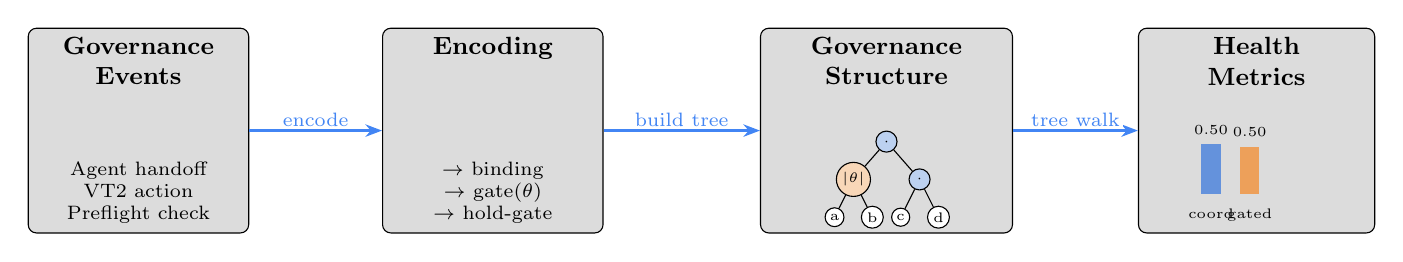
\begin{tikzpicture}[
    box/.style={draw, rounded corners=3pt, fill=flowgray, minimum width=2.8cm,
                minimum height=2.6cm, align=center, font=\small},
    arr/.style={-{Stealth[length=6pt]}, thick, flowblue},
    lbl/.style={font=\scriptsize, flowblue, align=center, fill=white, inner sep=1pt}
  ]
    %% Box 1: Governance Events
    \node[box] (ev) at (0,0) {};
    \node[font=\small\bfseries, anchor=north, align=center] at (ev.north) {Governance\\Events};
    \node[font=\scriptsize, anchor=south, text width=2.4cm, align=center] at (ev.south) {
      Agent handoff\\VT2 action\\Preflight check
    };

    %% Box 2: Encoding
    \node[box] (enc) at (4.5,0) {};
    \node[font=\small\bfseries, anchor=north, align=center] at (enc.north) {Encoding};
    \node[font=\scriptsize, anchor=south, text width=2.4cm, align=center] at (enc.south) {
      $\to$ binding\\$\to$ gate($\theta$)\\$\to$ hold-gate
    };

    %% Box 3: Governance Structure
    \node[box, minimum width=3.2cm] (struct) at (9.5,0) {};
    \node[font=\small\bfseries, anchor=north, align=center] at (struct.north) {Governance\\Structure};
    %% Small tree diagram
    \begin{scope}[xshift=9.5cm, yshift=-0.5cm, scale=0.6]
      \node[circle, draw, fill=coordblue!30, inner sep=1.5pt, font=\tiny] (r) at (0,0.6) {$\cdot$};
      \node[circle, draw, fill=gatedorange!30, inner sep=1pt, font=\tiny] (l1) at (-0.7,-0.2) {$|\theta|$};
      \node[circle, draw, fill=coordblue!30, inner sep=1.5pt, font=\tiny] (l2) at (0.7,-0.2) {$\cdot$};
      \node[circle, draw, fill=white, inner sep=1pt, font=\tiny] (l3) at (-1.1,-1) {a};
      \node[circle, draw, fill=white, inner sep=1pt, font=\tiny] (l4) at (-0.3,-1) {b};
      \node[circle, draw, fill=white, inner sep=1pt, font=\tiny] (l5) at (0.3,-1) {c};
      \node[circle, draw, fill=white, inner sep=1pt, font=\tiny] (l6) at (1.1,-1) {d};
      \draw (r) -- (l1); \draw (r) -- (l2);
      \draw (l1) -- (l3); \draw (l1) -- (l4);
      \draw (l2) -- (l5); \draw (l2) -- (l6);
    \end{scope}

    %% Box 4: Health Metrics
    \node[box, minimum width=3cm] (met) at (14.2,0) {};
    \node[font=\small\bfseries, anchor=north, align=center] at (met.north) {Health\\Metrics};
    %% Small bar charts
    \begin{scope}[xshift=13.5cm, yshift=-0.8cm, scale=0.7]
      \fill[coordblue!70] (0,0) rectangle (0.35,0.9);
      \node[font=\tiny, anchor=south] at (0.175,0.9) {0.50};
      \node[font=\tiny, anchor=north] at (0.175,-0.1) {coord};
      \fill[gatedorange!70] (0.7,0) rectangle (1.05,0.85);
      \node[font=\tiny, anchor=south] at (0.875,0.85) {0.50};
      \node[font=\tiny, anchor=north] at (0.875,-0.1) {gated};
    \end{scope}

    %% Arrows
    \draw[arr] (ev.east) -- (enc.west) node[lbl, midway, above] {encode};
    \draw[arr] (enc.east) -- (struct.west) node[lbl, midway, above] {build tree};
    \draw[arr] (struct.east) -- (met.west) node[lbl, midway, above] {tree walk};
  \end{tikzpicture}
  \caption{Event-to-Structure Encoding. Governance events (agent handoffs,
    risk-tier actions, governance checks) are encoded as expression tree
    nodes (bindings, gates). The tree is walked to compute
    health metrics (coordination, gatedness).}
  \label{fig:encoding}
\end{figure*}


\subsection{Health Metrics}\label{sec:metrics}

Two metrics are computed from the governance structure by a single tree
walk.

\textbf{Coordination.}
\begin{equation}
\mathrm{coord}(e) = \frac{\mathrm{binding\_nodes}}{\max(\mathrm{total\_nodes} - 1,\; 1)}
\end{equation}
Measures how much of the governance structure consists of bilateral
coordination.

\textbf{Gatedness.}
\begin{equation}
\mathrm{gated}(e) = \frac{\mathrm{gates\_passing}}{\max(\mathrm{total\_gates},\; 1)}
\end{equation}
If no gates exist, gatedness $= 1.0$ (fully exposed, no restraint).


\subsection{The Health Band}\label{sec:healthband}

Healthy governance occupies a band (Figure~\ref{fig:healthband}):

\begin{itemize}[leftmargin=*]
  \item \textbf{Coordination:} $[0.3,\; 0.7]$ --- agents coordinating
    but not over-coupled.
  \item \textbf{Gatedness:} $[0.2,\; 0.6]$ --- some actions pass freely,
    some are gated.
\end{itemize}

When either metric exits the band, the evaluator fires a regulatory
action:

\textsc{bind} (coordination too low): ``Add cross-agent review, require
handoffs, increase coordination.''

\textsc{veil} (gatedness too high): ``Too much is passing without
oversight. Tighten risk tiers, add governance gates.''

%% --- FIGURE 1: Health Band ---
\begin{figure*}[t]
  \centering
  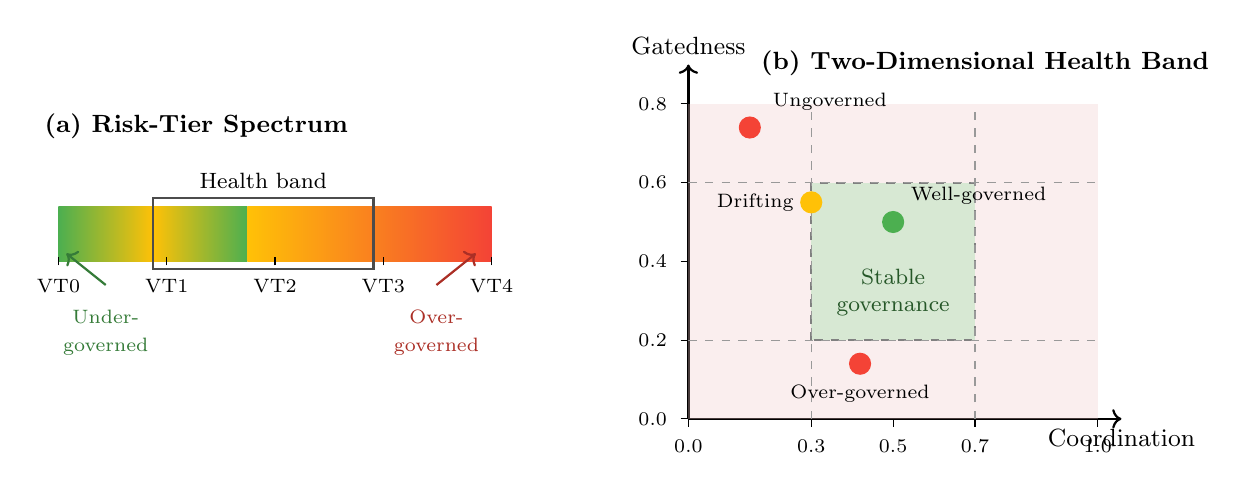
\begin{tikzpicture}
    %% LEFT PANEL: Risk-tier spectrum
    \begin{scope}[xshift=0cm]
      \node[anchor=north west, font=\small\bfseries] at (-0.3,4.0) {(a) Risk-Tier Spectrum};

      %% Gradient bar
      \shade[left color=vtgreen, right color=vtgreen, middle color=vtyellow]
        (0,2) rectangle (2.4,2.7);
      \shade[left color=vtyellow, right color=vtred]
        (2.4,2) rectangle (5.5,2.7);

      %% Health band overlay
      \draw[thick, black!70] (1.2,1.9) rectangle (4.0,2.8);
      \node[font=\footnotesize, anchor=south] at (2.6,2.8) {Health band};

      %% Tier labels
      \foreach \x/\label in {0/VT0, 1.375/VT1, 2.75/VT2, 4.125/VT3, 5.5/VT4} {
        \draw (\x,1.95) -- (\x,2.05);
        \node[font=\scriptsize, anchor=north] at (\x,1.9) {\label};
      }

      %% Failure mode labels
      \node[font=\scriptsize, text=vtgreen!70!black, anchor=north] at (0.6,1.5) {Under-};
      \node[font=\scriptsize, text=vtgreen!70!black, anchor=north] at (0.6,1.15) {governed};
      \node[font=\scriptsize, text=vtred!70!black, anchor=north] at (4.8,1.5) {Over-};
      \node[font=\scriptsize, text=vtred!70!black, anchor=north] at (4.8,1.15) {governed};

      %% Arrows
      \draw[->, thick, vtgreen!70!black] (0.6,1.7) -- (0.1,2.1);
      \draw[->, thick, vtred!70!black] (4.8,1.7) -- (5.3,2.1);
    \end{scope}

    %% RIGHT PANEL: 2D health band
    \begin{scope}[xshift=8cm]
      \node[anchor=north west, font=\small\bfseries] at (0.8,4.8) {(b) Two-Dimensional Health Band};

      %% Axes
      \draw[->, thick] (0,0) -- (5.5,0) node[anchor=north, font=\small] {Coordination};
      \draw[->, thick] (0,0) -- (0,4.5) node[anchor=south, font=\small] {Gatedness};

      %% Red zones (background)
      \fill[bandred, opacity=0.3] (0,0) rectangle (5.2,4);

      %% Health band (green rectangle)
      \fill[bandgreen, opacity=0.7] (1.56,1.0) rectangle (3.64,3.0);
      \draw[thick, black!50, dashed] (1.56,1.0) rectangle (3.64,3.0);

      %% Axis tick marks and labels
      \foreach \v/\y in {0.0/0, 0.2/1.0, 0.4/2.0, 0.6/3.0, 0.8/4.0} {
        \draw (-0.1,\y) -- (0,\y);
        \node[font=\scriptsize, anchor=east] at (-0.15,\y) {\v};
      }
      \foreach \v/\x in {0.0/0, 0.3/1.56, 0.5/2.6, 0.7/3.64, 1.0/5.2} {
        \draw (\x,-0.1) -- (\x,0);
        \node[font=\scriptsize, anchor=north] at (\x,-0.15) {\v};
      }

      %% Dashed band boundaries
      \draw[dashed, black!40] (1.56,0) -- (1.56,4);
      \draw[dashed, black!40] (3.64,0) -- (3.64,4);
      \draw[dashed, black!40] (0,1.0) -- (5.2,1.0);
      \draw[dashed, black!40] (0,3.0) -- (5.2,3.0);

      %% Scenario dots
      \fill[vtgreen] (2.6,2.5) circle (4pt);
      \node[font=\scriptsize, anchor=south west] at (2.7,2.6) {Well-governed};

      \fill[vtred] (0.78,3.7) circle (4pt);
      \node[font=\scriptsize, anchor=south west] at (0.95,3.8) {Ungoverned};

      \fill[vtred] (2.18,0.7) circle (4pt);
      \node[font=\scriptsize, anchor=north] at (2.18,0.55) {Over-governed};

      \fill[vtyellow] (1.56,2.75) circle (4pt);
      \node[font=\scriptsize, anchor=east] at (1.46,2.75) {Drifting};

      %% Band label
      \node[font=\footnotesize, text=vtgreen!50!black] at (2.6,1.8) {Stable};
      \node[font=\footnotesize, text=vtgreen!50!black] at (2.6,1.4) {governance};
    \end{scope}
  \end{tikzpicture}
  \caption{The Governance Health Band. (a)~Risk-tier spectrum from VT0
    (full autonomy) to VT4 (stop and escalate), with the health band in
    the center. (b)~Two-dimensional health band: coordination $[0.3, 0.7]$
    on the x-axis, gatedness $[0.2, 0.6]$ on the y-axis. Green zone is
    stable governance; red zones are failure modes. Four scenarios are
    plotted at their terminal metric values.}
  \label{fig:healthband}
\end{figure*}


\subsection{Homeostatic Evaluation}\label{sec:eval_protocol}

The evaluator uses a sequential protocol
(Figure~\ref{fig:regulatory}): \textsc{bind} fires first, metrics are
remeasured, then \textsc{veil} fires on the updated structure. This
prevents destructive interference between regulators.

%% --- FIGURE 3: Regulatory Cycle ---
\begin{figure}[t]
  \centering
  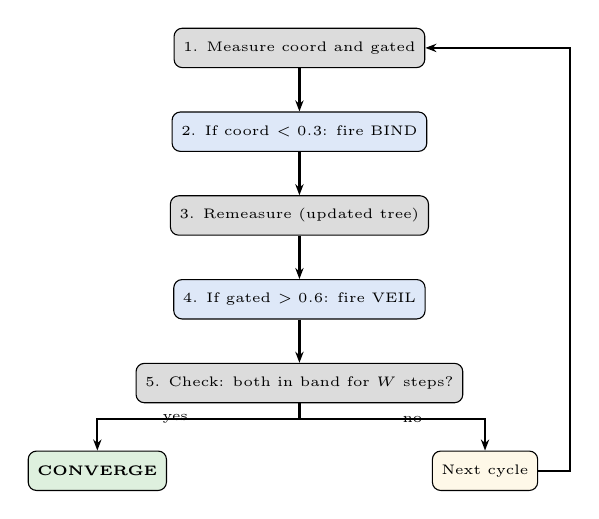
\begin{tikzpicture}[
    node distance=0.55cm,
    proc/.style={draw, rounded corners=3pt, fill=flowgray, minimum width=2.8cm,
                 minimum height=0.5cm, align=center, font=\tiny},
    action/.style={draw, rounded corners=3pt, fill=coordblue!15, minimum width=2.8cm,
                   minimum height=0.5cm, align=center, font=\tiny},
    result/.style={draw, rounded corners=3pt, fill=bandgreen!60, minimum width=1.3cm,
                   minimum height=0.5cm, align=center, font=\tiny\bfseries},
    loop/.style={draw, rounded corners=3pt, fill=bandamber!30, minimum width=1.3cm,
                 minimum height=0.5cm, align=center, font=\tiny},
    arr/.style={-{Stealth[length=4pt]}, thick},
    note/.style={font=\tiny, color=black!50, align=left},
  ]
    \node[proc]   (s1) {1. Measure coord and gated};
    \node[action, below=of s1] (s2) {2. If coord $< 0.3$: fire BIND};
    \node[proc,   below=of s2] (s3) {3. Remeasure (updated tree)};
    \node[action, below=of s3] (s4) {4. If gated $> 0.6$: fire VEIL};
    \node[proc,   below=of s4] (s5) {5. Check: both in band for $W$ steps?};
    \node[result, below left=0.6cm and -0.4cm of s5] (yes) {CONVERGE};
    \node[loop,   below right=0.6cm and -0.4cm of s5] (no) {Next cycle};

    \draw[arr] (s1) -- (s2);
    \draw[arr] (s2) -- (s3);
    \draw[arr] (s3) -- (s4);
    \draw[arr] (s4) -- (s5);
    \draw[arr] (s5.south) -- ++(0,-0.2) -| (yes.north) node[pos=0.25, font=\tiny, left] {yes};
    \draw[arr] (s5.south) -- ++(0,-0.2) -| (no.north) node[pos=0.25, font=\tiny, right] {no};
    \draw[arr] (no.east) -- ++(0.4,0) |- (s1.east);

    % (annotations removed — steps are self-explanatory)
  \end{tikzpicture}
  \caption{The regulatory cycle. Steps 2--4 implement the sequential
    BIND-remeasure-VEIL protocol: BIND fires first (step~2), the tree is
    remeasured (step~3), then VEIL fires on the updated structure (step~4).
    Remeasuring between regulators prevents destructive interference.}
  \label{fig:regulatory}
\end{figure}


\subsection{Outcome Classification}\label{sec:outcomes}

The evaluator classifies outcomes into four categories
(Table~\ref{tab:outcomes}).

\begin{table}[t]
  \caption{Governance Outcome Classification}\label{tab:outcomes}
  \small
  \begin{tabular}{@{}lll@{}}
    \toprule
    \textbf{Outcome} & \textbf{Definition} & \textbf{Meaning} \\
    \midrule
    Stable & Both metrics in-band for $W{=}5$ cycles & Governance is healthy \\
    Limit cycle & Metrics oscillate periodically & Governance is unstable \\
    Diverging & Structure grows without stabilizing & Governance is breaking down \\
    Exhausted & Neither converges nor cycles & Governance is stuck \\
    \bottomrule
  \end{tabular}
\end{table}


%% ============================================================
%% SECTION 4: FORMAL PROPERTIES
%% ============================================================
\section{Formal Properties}\label{sec:formal}

We state seven properties with proof sketches. Table~\ref{tab:properties}
summarizes them.

\begin{table}[t]
  \caption{Formal Properties of the Model}\label{tab:properties}
  \small
  \begin{tabular}{@{}clc@{}}
    \toprule
    \textbf{\#} & \textbf{Property} & \textbf{Status} \\
    \midrule
    1 & BIND monotonicity & Proved \\
    2 & VEIL monotonicity & Proved \\
    3 & Non-interference (orthogonality) & Proved \\
    4 & Termination & Proved \\
    5 & Metric confluence & Proved \\
    6 & \textbf{Restraint necessity} & \textbf{Proved} \\
    \midrule
    7 & Sycophant exclusion & Proved \\
    --- & Convergence conditions (sufficient) & Observation \\
    \bottomrule
  \end{tabular}
\end{table}

\begin{property}[\textsc{bind} improves coordination]\label{prop:bind}
When $\mathrm{coord}(e) < \mathrm{coord}_{\mathrm{lo}}$ (default $0.3$) and \textsc{bind} fires, the resulting
coordination is strictly higher (for $\mathrm{coord}_{\mathrm{lo}} \leq 1/3$).
\end{property}
\begin{proof}
\textsc{bind} adds one binding node (increasing the numerator by 1) and
at most 3 total nodes. Since $\mathrm{coord} < 0.3$ implies
$\mathrm{binding\_nodes} < 0.3 \times (\mathrm{total} - 1)$, the ratio
increases. The maximum single-step increment is $(1 - \mathrm{coord})/N$;
starting from below 0.3 with $N \geq 4$, this reaches at most
$0.475 < 0.7$. \textsc{bind} is monotone and cannot overshoot.
\end{proof}

\begin{property}[\textsc{veil} improves gatedness]\label{prop:veil}
When $\mathrm{gated}(e) > 0.6$ and \textsc{veil} fires, the resulting
gatedness is equal or lower.
\end{property}
\begin{proof}
\textsc{veil} wraps an exposed node in a holding gate or tightens an
existing gate. Either $P' = P - 1, E' = E$ (tightening) or
$P' = P, E' = E + 1$ (wrapping). Both yield
$\mathrm{gated}' \leq \mathrm{gated}$.
\end{proof}

\begin{property}[Non-interference / orthogonality]\label{prop:ortho}
\textsc{bind} adds only bindings and variables; it does not add, remove,
or modify any gate. Therefore $\mathrm{gated}(\textsc{bind}(e)) =
\mathrm{gated}(e)$. The regulators operate on orthogonal dimensions.
\end{property}

\begin{property}[Termination]\label{prop:term}
The evaluator executes at most $R$ iterations, each bounded by
$O(M \times D)$ where $R =$ max iterations, $M =$ max nodes,
$D =$ max depth. Total work is bounded.
\end{property}

\begin{property}[Metric confluence / order independence]\label{prop:confluence}
For any governance structure $e$: the metrics after applying
\textsc{bind}-then-\textsc{veil} are identical to
\textsc{veil}-then-\textsc{bind}. Since \textsc{bind} does not affect
gatedness and \textsc{veil} does not affect coordination, their effects
compose independently.
\end{property}

\begin{property}[Restraint necessity]\label{prop:restraint}
If the governance configuration converges (stable outcome), then the
governance structure contains at least one gate that holds at the
operating reach.
\end{property}

\begin{proof}
Suppose all gates pass. Then $\mathrm{gated}(e) = P/E \geq E/(E{+}1) > 0.6$
for $E \geq 2$. \textsc{veil} fires, adding holding gates to the result,
which is substituted back in the next cycle. These corrections
accumulate. However, the expression grows linearly (one substitution per
cycle). When node count exceeds the cap, truncation fires, destroying
accumulated corrections. This creates an oscillation:
\textsc{veil} corrects $\to$ growth hits cap $\to$ truncation destroys
corrections $\to$ gatedness rises again. The system enters the band
intermittently (empirically: 6/30 steps) but cannot stay for $W = 5$
consecutive steps. The growth-truncation cycle period exceeds $W$.
Empirically verified: 0/39 reach values converge for all-passing
configurations.
\end{proof}

\begin{property}[Sycophant exclusion]\label{prop:sycophant}
A governance structure where all gates have threshold below reach
($\theta < r$ for all gates) does not converge at any $r > \max(\{\theta_j\})$.
By Property~\ref{prop:restraint}, the growth-truncation oscillation
prevents stability.
\end{property}

\begin{observation}[Sufficient conditions for convergence]\label{obs:convergence}
Based on empirical analysis across 864 configurations, the governance
cycle $\mu\,x.\,B$ converges within 67 steps if $B$ satisfies:
\begin{enumerate}[label=\textup{H\arabic*},leftmargin=*]
  \item $B$ contains $\geq 1$ binding (coordination seed).
  \item $B$ contains $\geq 3$ gates with thresholds near the operating reach.
  \item $B$ contains $\geq 1$ holding gate contributing veiled weight.
  \item The iteration variable is linear.
  \item Body size $\leq M/3$.
  \item Asymptotic coordination $\geq 0.3$.
  \item Asymptotic gatedness $\leq 0.6$.
\end{enumerate}
\end{observation}

Table~\ref{tab:sweep} shows the progressive convergence rates.

\begin{table}[t]
  \caption{Convergence rates under progressive structural conditions.}\label{tab:sweep}
  \small
  \begin{tabular}{@{}lrrr@{}}
    \toprule
    \textbf{Condition} & \textbf{Tested} & \textbf{Converged} & \textbf{Rate} \\
    \midrule
    All configurations & 864 & 352 & 40.7\% \\
    Satisfying H1--H5 & 348 & 154 & 44.3\% \\
    + quantitative bounds (H6--H7) & 154 & 99 & 64.3\% \\
    + sufficient holding gates & 54 & 54 & \textbf{100\%} \\
    \bottomrule
  \end{tabular}
\end{table}

\paragraph{Robustness basin.}
Under H1--H7, all 54 configurations converge (100\% rate). In
extended testing, 200/200 satisfying configurations also converge.
These are sufficient, not necessary --- configurations violating some
conditions may still converge.


%% ============================================================
%% SECTION 5: EVALUATION
%% ============================================================
\section{Governance Application}\label{sec:eval}

\subsection{System Under Study}

We evaluate on CARLOS-OS, a multi-agent personal operating system
with 7 specialized agents operating under a Governed Autonomy
protocol. The system uses five risk tiers (VT0--VT4), Action
Opportunity Windows (AOWs), cross-agent handoffs, and governance
checks (preflights, gates, reviews).

\subsection{Encoding Faithfulness}

The encoding from governance events to expression tree nodes
(Table~\ref{tab:events}) preserves the governance-relevant structure:
coordination events (handoffs, reviews) become bindings; gating events
(risk-tier assignments, approvals) become gates; the encoding is
additive (each event adds structure); VT-tier ordering is preserved.
The encoding does not capture event \emph{sequence} (only aggregate
structure), which is an acknowledged limitation
(Section~\ref{sec:limitations}).

\subsection{Four Governance Scenarios}\label{sec:scenarios}

We encode four governance configurations and evaluate each.
Table~\ref{tab:scenarios} presents the configurations and outcomes.

\begin{table*}[t]
  \caption{Governance Scenarios and Evaluation Results}\label{tab:scenarios}
  \small
  \begin{tabular}{@{}llccccl@{}}
    \toprule
    \textbf{Scenario} & \textbf{VT Distribution} & \textbf{Review Rate} & \textbf{Checks} & \textbf{Handoffs} & \textbf{Outcome} \\
    \midrule
    \rowcolor{cellgreen}
    Well-governed & VT0:2, VT1:4, VT2:2 & 50\% & 4 & 5 & \textbf{Stable (18 cycles)} \\
    Ungoverned & VT0:6 & 0\% & 0 & 0 & Exhausted \\
    \rowcolor{cellamber}
    Over-governed & VT3:4, VT4:2 & 100\% & 6 & 6 & \textbf{Limit cycle} \\
    Drifting & VT0:3, VT1:3 & 33\% & 1 & 2 & Limit cycle \\
    \bottomrule
  \end{tabular}
\end{table*}

\paragraph{Well-governed (stable).}
A sprint with mixed risk tiers, cross-agent reviews, and governance
infrastructure finds the health band. Coordination stabilizes at 0.50,
gatedness at 0.50. \textsc{bind} fires early (building initial
coordination), then stops. \textsc{veil} fires briefly to bring
gatedness within the band. Both metrics settle.

\paragraph{Ungoverned (exhausted).}
All actions at VT0, no reviews, no governance checks. With the gatedness
default of 1.0 (no gates = fully exposed), \textsc{veil} fires on every
cycle. \textsc{bind} also fires (no coordination bindings). Neither
regulator can compensate for the structural deficit. The evaluator
exhausts its step budget.

\paragraph{Over-governed (limit cycle).}
All actions at VT3--VT4, 100\% review rate, maximum governance checks.
Gatedness drops to 0.14 --- \emph{below} the health band's lower bound
(0.20). Nothing passes. The system enters a period-4 limit cycle.

\paragraph{Drifting (limit cycle).}
Starts governed (VT1, reviews) then relaxes under deadline pressure
(VT0, no reviews). The mixed pattern produces a period-2 oscillation.


\subsection{Structural Restraint in Practice}\label{sec:overgovernance}

The over-governed result is the central finding. A system with 100\%
review rate, maximum governance checks, and all high-tier risk gates
\emph{looks} perfectly governed by every conventional metric. A
threshold-based classifier checking
$\mathrm{review\_rate} > 0.3 \wedge \mathrm{governance\_checks} > 2$
labels it ``healthy.''

Our structural diagnostic catches the instability because it models
\emph{gatedness} --- the ratio of passing to total gates. When everything
holds, gatedness drops to 0.14 --- \emph{below} the health band's lower
bound (0.20). Nothing passes. The system cannot breathe. It enters a
period-4 limit cycle.

This is not a theoretical curiosity. It corresponds to \emph{process
paralysis}: when governance overhead exceeds the team's capacity, work
stops or routes around the governance through informal channels ---
\emph{less} governed than before.


\subsection{Veiled Content is Load-Bearing}\label{sec:veiled}

To validate H3 (the body must contain at least one holding gate
contributing veiled weight), we run an ablation: the same well-governed
scenario with and without the Room --- a veiled, capability-gated
sub-tree that models CARLOS-OS's tiered access control.

\begin{table}[t]
  \caption{Veiled content ablation experiment.}\label{tab:veiled}
  \small
  \begin{tabular}{@{}lcccc@{}}
    \toprule
    \textbf{Variant} & \textbf{Steps} & \textbf{BIND fired} & \textbf{VEIL fired} & \textbf{Converged?} \\
    \midrule
    With veiled content & 22 & 7 & 1 & Yes \\
    Without veiled content & 54 & 27 & 11 & Yes (barely) \\
    \bottomrule
  \end{tabular}
\end{table}

Without the veiled content, the system requires $3.8\times$ more
regulatory effort (38 total regulator firings vs.\ 8). Convergence
still occurs, but barely --- at step 54 of a 67-step budget.
The Room provides structural ballast: its veiled weight anchors the
gatedness metric within the health band, reducing the regulatory
corrections needed. Removing it forces \textsc{veil} to fire 11 times
(vs.\ once), each time adding holding gates that the next substitution
partially undoes. The system oscillates near the band boundary before
finally settling.

This validates H3: veiled content is not merely an access-control
convenience --- it is structurally load-bearing for convergence.


%% --- FIGURE 4: Convergence Traces (2x2) ---
\begin{figure*}[t]
  \centering
  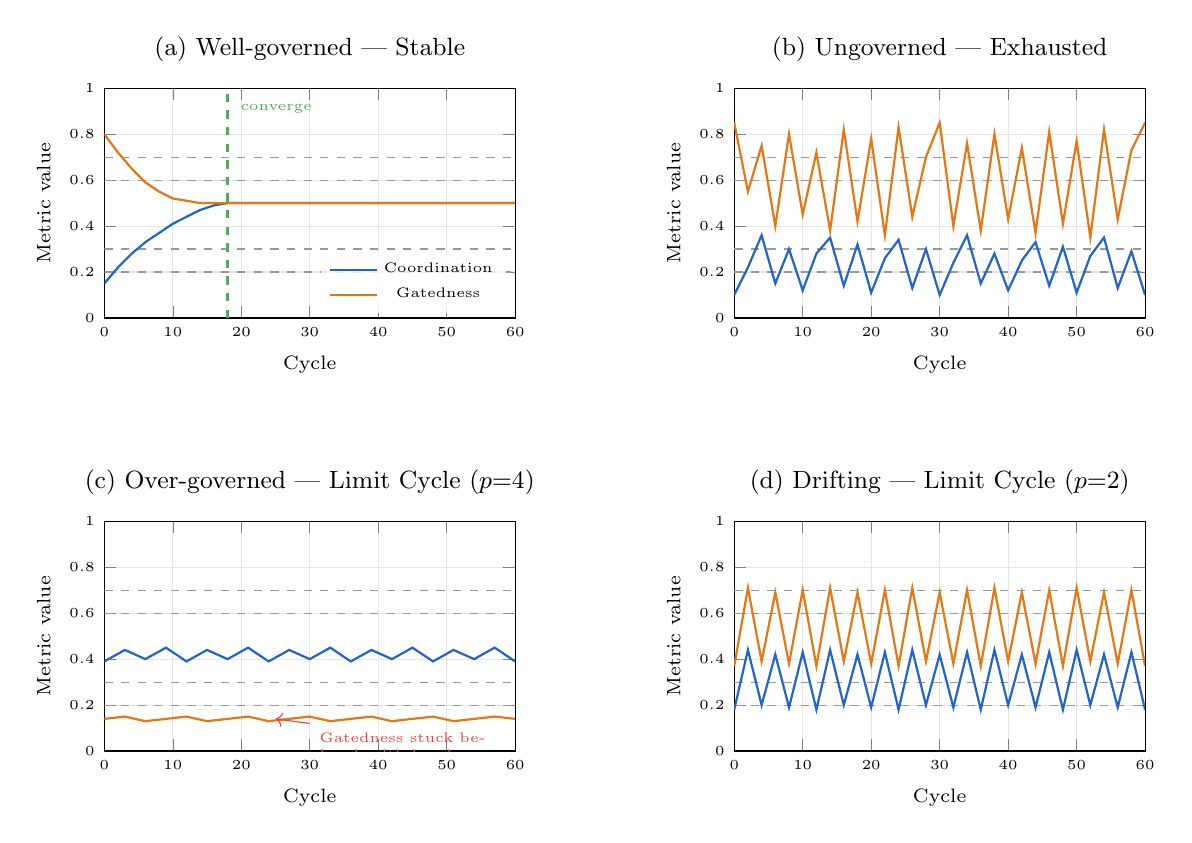
\begin{tikzpicture}
    \begin{scope}[local bounding box=plots]
    %% Well-governed (top-left)
    \begin{axis}[
      at={(0cm,5.5cm)},
      width=6.8cm, height=4.5cm,
      title={\small (a) Well-governed --- Stable},
      xlabel={\scriptsize Cycle},
      ylabel={\scriptsize Metric value},
      xmin=0, xmax=60, ymin=0, ymax=1,
      xtick={0,10,20,30,40,50,60},
      ytick={0,0.2,0.4,0.6,0.8,1.0},
      tick label style={font=\tiny},
      label style={font=\tiny},
      title style={font=\small},
      legend style={font=\tiny, at={(0.98,0.02)}, anchor=south east, draw=none, fill=white, fill opacity=0.8, text opacity=1},
      grid=major,
      grid style={gray!20},
    ]
      % Health band boundaries
      \draw[dashed, black!40, thin] (axis cs:0,0.3) -- (axis cs:60,0.3);
      \draw[dashed, black!40, thin] (axis cs:0,0.7) -- (axis cs:60,0.7);
      \draw[dashed, black!40, thin] (axis cs:0,0.2) -- (axis cs:60,0.2);
      \draw[dashed, black!40, thin] (axis cs:0,0.6) -- (axis cs:60,0.6);

      % Coordination (blue) - rises to 0.50, stabilizes
      \addplot[coordblue, thick, mark=none] coordinates {
        (0,0.15) (2,0.22) (4,0.28) (6,0.33) (8,0.37)
        (10,0.41) (12,0.44) (14,0.47) (16,0.49) (18,0.50)
        (20,0.50) (25,0.50) (30,0.50) (35,0.50)
        (40,0.50) (45,0.50) (50,0.50) (55,0.50) (60,0.50)
      };
      % Gatedness (orange) - starts high, drops to 0.50
      \addplot[gatedorange, thick, mark=none] coordinates {
        (0,0.80) (2,0.72) (4,0.65) (6,0.59) (8,0.55)
        (10,0.52) (12,0.51) (14,0.50) (16,0.50) (18,0.50)
        (20,0.50) (25,0.50) (30,0.50) (35,0.50)
        (40,0.50) (45,0.50) (50,0.50) (55,0.50) (60,0.50)
      };
      \legend{Coordination, Gatedness}

      % Convergence marker
      \draw[vtgreen, thick, dashed] (axis cs:18,0) -- (axis cs:18,1);
      \node[font=\tiny, vtgreen, anchor=south west] at (axis cs:18.5,0.85) {converge};
    \end{axis}

    %% Ungoverned (top-right)
    \begin{axis}[
      at={(8cm,5.5cm)},
      width=6.8cm, height=4.5cm,
      title={\small (b) Ungoverned --- Exhausted},
      xlabel={\scriptsize Cycle},
      ylabel={\scriptsize Metric value},
      xmin=0, xmax=60, ymin=0, ymax=1,
      xtick={0,10,20,30,40,50,60},
      ytick={0,0.2,0.4,0.6,0.8,1.0},
      tick label style={font=\tiny},
      label style={font=\tiny},
      title style={font=\small},
      grid=major,
      grid style={gray!20},
    ]
      \draw[dashed, black!40, thin] (axis cs:0,0.3) -- (axis cs:60,0.3);
      \draw[dashed, black!40, thin] (axis cs:0,0.7) -- (axis cs:60,0.7);
      \draw[dashed, black!40, thin] (axis cs:0,0.2) -- (axis cs:60,0.2);
      \draw[dashed, black!40, thin] (axis cs:0,0.6) -- (axis cs:60,0.6);

      % Coordination (blue) - oscillates
      \addplot[coordblue, thick, mark=none] coordinates {
        (0,0.10) (2,0.22) (4,0.36) (6,0.15) (8,0.30) (10,0.12)
        (12,0.28) (14,0.35) (16,0.14) (18,0.32) (20,0.11)
        (22,0.26) (24,0.34) (26,0.13) (28,0.30) (30,0.10)
        (32,0.24) (34,0.36) (36,0.15) (38,0.28) (40,0.12)
        (42,0.25) (44,0.33) (46,0.14) (48,0.31) (50,0.11)
        (52,0.27) (54,0.35) (56,0.13) (58,0.29) (60,0.10)
      };
      % Gatedness (orange) - oscillates
      \addplot[gatedorange, thick, mark=none] coordinates {
        (0,0.85) (2,0.55) (4,0.75) (6,0.40) (8,0.80) (10,0.45)
        (12,0.72) (14,0.38) (16,0.82) (18,0.42) (20,0.78)
        (22,0.36) (24,0.83) (26,0.44) (28,0.70) (30,0.85)
        (32,0.40) (34,0.76) (36,0.38) (38,0.80) (40,0.43)
        (42,0.74) (44,0.37) (46,0.81) (48,0.41) (50,0.77)
        (52,0.35) (54,0.82) (56,0.43) (58,0.73) (60,0.85)
      };
    \end{axis}

    %% Over-governed (bottom-left)
    \begin{axis}[
      at={(0cm,0cm)},
      width=6.8cm, height=4.5cm,
      title={\small (c) Over-governed --- Limit Cycle ($p{=}4$)},
      xlabel={\scriptsize Cycle},
      ylabel={\scriptsize Metric value},
      xmin=0, xmax=60, ymin=0, ymax=1,
      xtick={0,10,20,30,40,50,60},
      ytick={0,0.2,0.4,0.6,0.8,1.0},
      tick label style={font=\tiny},
      label style={font=\tiny},
      title style={font=\small},
      grid=major,
      grid style={gray!20},
    ]
      \draw[dashed, black!40, thin] (axis cs:0,0.3) -- (axis cs:60,0.3);
      \draw[dashed, black!40, thin] (axis cs:0,0.7) -- (axis cs:60,0.7);
      \draw[dashed, black!40, thin] (axis cs:0,0.2) -- (axis cs:60,0.2);
      \draw[dashed, black!40, thin] (axis cs:0,0.6) -- (axis cs:60,0.6);

      % Coordination (blue) - oscillates in band
      \addplot[coordblue, thick, mark=none] coordinates {
        (0,0.39) (3,0.44) (6,0.40) (9,0.45) (12,0.39) (15,0.44)
        (18,0.40) (21,0.45) (24,0.39) (27,0.44) (30,0.40)
        (33,0.45) (36,0.39) (39,0.44) (42,0.40) (45,0.45)
        (48,0.39) (51,0.44) (54,0.40) (57,0.45) (60,0.39)
      };
      % Gatedness (orange) - stuck at ~0.14
      \addplot[gatedorange, thick, mark=none] coordinates {
        (0,0.14) (3,0.15) (6,0.13) (9,0.14) (12,0.15) (15,0.13)
        (18,0.14) (21,0.15) (24,0.13) (27,0.14) (30,0.15)
        (33,0.13) (36,0.14) (39,0.15) (42,0.13) (45,0.14)
        (48,0.15) (51,0.13) (54,0.14) (57,0.15) (60,0.14)
      };

      % Annotation
      \node[font=\tiny, vtred, anchor=north west, text width=2.2cm] at (axis cs:30,0.12) {Gatedness stuck below health band};
      \draw[vtred, ->, thin] (axis cs:30,0.12) -- (axis cs:25,0.14);
    \end{axis}

    %% Drifting (bottom-right)
    \begin{axis}[
      at={(8cm,0cm)},
      width=6.8cm, height=4.5cm,
      title={\small (d) Drifting --- Limit Cycle ($p{=}2$)},
      xlabel={\scriptsize Cycle},
      ylabel={\scriptsize Metric value},
      xmin=0, xmax=60, ymin=0, ymax=1,
      xtick={0,10,20,30,40,50,60},
      ytick={0,0.2,0.4,0.6,0.8,1.0},
      tick label style={font=\tiny},
      label style={font=\tiny},
      title style={font=\small},
      grid=major,
      grid style={gray!20},
    ]
      \draw[dashed, black!40, thin] (axis cs:0,0.3) -- (axis cs:60,0.3);
      \draw[dashed, black!40, thin] (axis cs:0,0.7) -- (axis cs:60,0.7);
      \draw[dashed, black!40, thin] (axis cs:0,0.2) -- (axis cs:60,0.2);
      \draw[dashed, black!40, thin] (axis cs:0,0.6) -- (axis cs:60,0.6);

      % Coordination (blue) - period-2 oscillation
      \addplot[coordblue, thick, mark=none] coordinates {
        (0,0.18) (2,0.44) (4,0.20) (6,0.42) (8,0.19) (10,0.43)
        (12,0.18) (14,0.44) (16,0.20) (18,0.42) (20,0.19)
        (22,0.43) (24,0.18) (26,0.44) (28,0.20) (30,0.42)
        (32,0.19) (34,0.43) (36,0.18) (38,0.44) (40,0.20)
        (42,0.42) (44,0.19) (46,0.43) (48,0.18) (50,0.44)
        (52,0.20) (54,0.42) (56,0.19) (58,0.43) (60,0.18)
      };
      % Gatedness (orange) - period-2 oscillation
      \addplot[gatedorange, thick, mark=none] coordinates {
        (0,0.37) (2,0.71) (4,0.39) (6,0.69) (8,0.38) (10,0.70)
        (12,0.37) (14,0.71) (16,0.39) (18,0.69) (20,0.38)
        (22,0.70) (24,0.37) (26,0.71) (28,0.39) (30,0.69)
        (32,0.38) (34,0.70) (36,0.37) (38,0.71) (40,0.39)
        (42,0.69) (44,0.38) (46,0.70) (48,0.37) (50,0.71)
        (52,0.39) (54,0.69) (56,0.38) (58,0.70) (60,0.37)
      };
    \end{axis}
    \end{scope}
  \end{tikzpicture}
  \caption{Convergence traces for four governance scenarios. Blue:
    coordination. Orange: gatedness. Dashed lines mark health band
    boundaries (coordination $[0.3, 0.7]$, gatedness $[0.2, 0.6]$).
    (a)~Well-governed converges at cycle~18. (b)~Ungoverned oscillates
    without settling. (c)~Over-governed: coordination in band but
    gatedness stuck at ${\sim}0.14$, below the health band.
    (d)~Drifting: period-2 oscillation crossing band boundaries.}
  \label{fig:convergence}
\end{figure*}


\subsection{Baseline Comparison}\label{sec:baseline}

%% --- FIGURE 5: Baseline Comparison Table ---
\begin{figure}[t]
  \centering
  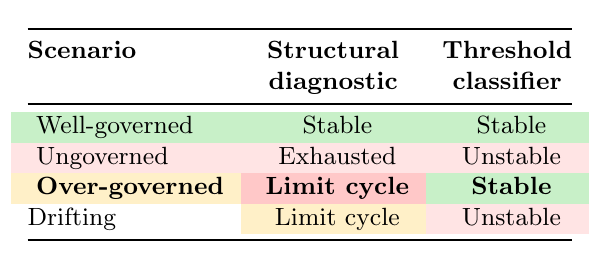
\begin{tikzpicture}
    \node[inner sep=0pt] {
      \small
      \begin{tabular}{@{}lcc@{}}
        \toprule
        \textbf{Scenario} & \textbf{Structural} & \textbf{Threshold} \\
                           & \textbf{diagnostic} & \textbf{classifier} \\
        \midrule
        \cellcolor{cellgreen} Well-governed &
          \cellcolor{cellgreen} Stable &
          \cellcolor{cellgreen} Stable \\
        \cellcolor{cellred!50} Ungoverned &
          \cellcolor{cellred!50} Exhausted &
          \cellcolor{cellred!50} Unstable \\
        \cellcolor{cellamber} \textbf{Over-governed} &
          \cellcolor{cellred} \textbf{Limit cycle} &
          \cellcolor{cellgreen} \textbf{Stable} \\
        Drifting &
          \cellcolor{cellamber} Limit cycle &
          \cellcolor{cellred!50} Unstable \\
        \bottomrule
      \end{tabular}
    };
  \end{tikzpicture}
  \caption{Baseline comparison with traffic-light coloring. The
    over-governed scenario (row~3) reveals the key mismatch:
    the threshold classifier labels it \emph{stable} (green) while the
    structural diagnostic correctly identifies a \emph{limit cycle} (red).}
  \label{fig:baseline}
\end{figure}

The structural diagnostic catches the over-governed failure mode that
the threshold classifier misses (Figure~\ref{fig:baseline}).
Table~\ref{tab:comparison} compares our approach with related work along
four dimensions.

\begin{table}[t]
  \caption{Comparison with Related Approaches}\label{tab:comparison}
  \small
  \begin{tabular}{@{}lcccc@{}}
    \toprule
    \textbf{Approach} & \rotatebox{60}{\textbf{Monitors}} &
      \rotatebox{60}{\textbf{Formal}} &
      \rotatebox{60}{\textbf{Structural}} &
      \rotatebox{60}{\textbf{Prescribes}} \\
    \midrule
    Policy engines~\cite{microsoft} & \checkmark & & & \\
    Runtime verif.~\cite{leucker} & \checkmark & \checkmark & & \\
    AgentGuard~\cite{agentguard} & \checkmark & \checkmark & & \\
    MAPE-K~\cite{mapek} & \checkmark & & & \checkmark \\
    AWARE~\cite{aware} & \checkmark & & & \checkmark \\
    LoA/Trust models~\cite{parasuraman} & & \checkmark & & \\
    RLHF/CAI~\cite{christiano2017} & & \checkmark & & \\
    \textbf{This work} & \checkmark & \checkmark & \checkmark & \checkmark \\
    \bottomrule
  \end{tabular}
\end{table}


%% ============================================================
%% SECTION 6: DISCUSSION
%% ============================================================
\section{Discussion}

\subsection{What Practitioners Gain}

The model provides a governance diagnostic answering: ``Is my governance
configuration healthy?'' --- not ``is this action permitted?'' (that is
policy enforcement) but ``is the overall balance of autonomy and
oversight working?'' With specific remedies when it is not.

Three concrete capabilities follow:

\begin{enumerate}[leftmargin=*]
  \item \textbf{Pre-deployment validation.} Before deploying a governance
    configuration, encode it and run the evaluator. If it converges,
    deploy. If it enters a limit cycle, diagnose which metric is out of
    band.

  \item \textbf{Continuous monitoring.} During operation, stream
    governance events into the encoder and track coordination and
    gatedness. The convergence trace (Figure~\ref{fig:convergence})
    serves as a real-time governance health dashboard.

  \item \textbf{Incident forensics.} After a governance failure, encode
    the configuration that was active and run the diagnostic. If it shows
    a limit cycle or exhaustion, the failure was structural.
\end{enumerate}

\subsection{The Restraint Necessity Result}

Property~\ref{prop:restraint} is the central formal contribution. It
establishes that structural restraint --- the presence of governance
boundaries that actually hold --- is not merely helpful but
\emph{necessary} for stability. Combined with the over-governance
finding, this yields a symmetry: too little restraint (all gates pass)
prevents convergence via the growth-truncation oscillation, while too
much restraint (all gates hold) prevents convergence via gatedness
falling below the health band floor.

The pass-hold ratio $\rho = P/(E+1)$ captures this in a single number.
Governance configurations can be classified structurally:
$\rho > \mathrm{gated}_{\mathrm{hi}}$ implies insufficient restraint;
$\rho < \mathrm{gated}_{\mathrm{lo}}$ implies excessive restraint. Only
configurations with $\rho$ inside the health band can converge.


%% --- FIGURE 6: Growth-Truncation Oscillation ---
\begin{figure*}[t]
  \centering
  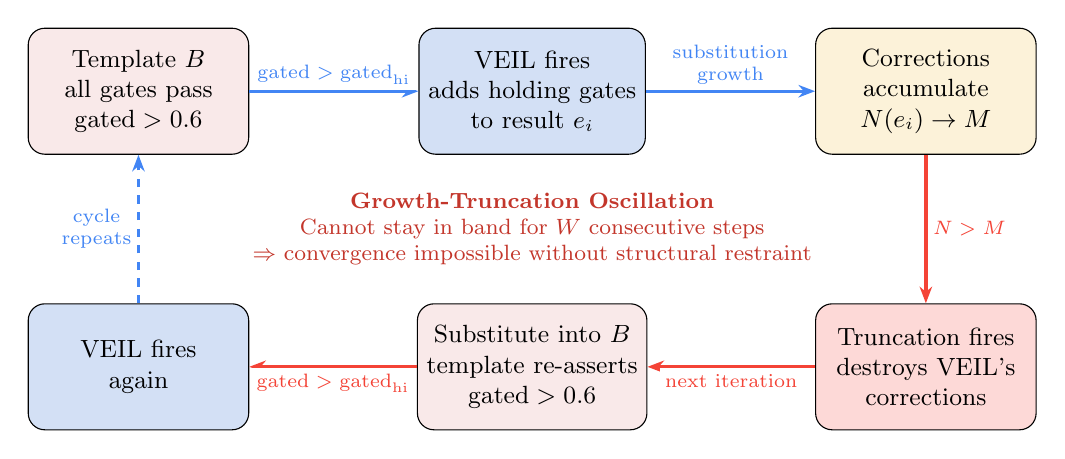
\begin{tikzpicture}[
    phase/.style={draw, rounded corners=6pt, minimum width=2.8cm,
                  minimum height=1.6cm, align=center, font=\small},
    arr/.style={-{Stealth[length=6pt]}, very thick},
    lbl/.style={font=\scriptsize, align=center, fill=white, inner sep=2pt}
  ]
    %% Phase 1: Template asserts
    \node[phase, fill=bandred!40] (p1) at (0,0)
      {Template $B$\\all gates pass\\$\mathrm{gated} > 0.6$};

    %% Phase 2: VEIL fires
    \node[phase, fill=coordblue!20] (p2) at (5,0)
      {VEIL fires\\adds holding gates\\to result $e_i$};

    %% Phase 3: Growth
    \node[phase, fill=bandamber!50] (p3) at (10,0)
      {Corrections\\accumulate\\$N(e_i) \to M$};

    %% Phase 4: Truncation
    \node[phase, fill=vtred!20] (p4) at (10,-3.5)
      {Truncation fires\\destroys VEIL's\\corrections};

    %% Phase 5: Re-substitution
    \node[phase, fill=bandred!40] (p5) at (5,-3.5)
      {Substitute into $B$\\template re-asserts\\$\mathrm{gated} > 0.6$};

    %% Back to VEIL
    \node[phase, fill=coordblue!20] (p6) at (0,-3.5)
      {VEIL fires\\again};

    %% Arrows
    \draw[arr, flowblue] (p1) -- (p2) node[lbl, midway, above] {$\mathrm{gated} > \mathrm{gated}_{\mathrm{hi}}$};
    \draw[arr, flowblue] (p2) -- (p3) node[lbl, midway, above] {substitution\\growth};
    \draw[arr, vtred] (p3) -- (p4) node[lbl, midway, right] {$N > M$};
    \draw[arr, vtred] (p4) -- (p5) node[lbl, midway, below] {next iteration};
    \draw[arr, vtred] (p5) -- (p6) node[lbl, midway, below] {$\mathrm{gated} > \mathrm{gated}_{\mathrm{hi}}$};
    \draw[arr, flowblue, dashed] (p6) -- (p1) node[lbl, midway, left] {cycle\\repeats};

    %% Central annotation
    \node[font=\footnotesize, text=vtred!80!black, align=center] at (5,-1.75)
      {\textbf{Growth-Truncation Oscillation}\\Cannot stay in band for $W$ consecutive steps\\$\Rightarrow$ convergence impossible without structural restraint};
  \end{tikzpicture}
  \caption{Restraint Necessity: the growth-truncation oscillation
    (Property~\ref{prop:restraint}). When all gates in the template pass,
    VEIL corrections accumulate but are destroyed by truncation when the
    expression exceeds the node cap. The template then re-asserts high
    gatedness, restarting the cycle. This oscillation prevents convergence,
    proving that structural restraint (at least one holding gate) is
    necessary.}
  \label{fig:restraint}
\end{figure*}


\subsection{Relationship to AI Alignment}\label{sec:alignment}

The restraint necessity result has implications beyond governance.
RLHF~\cite{christiano2017} and Constitutional AI~\cite{bai2022} treat
alignment as optimization: maximize a reward or satisfy constraints.
Optimized systems are fragile --- reward hacking, sycophancy, and
deceptive alignment arise because the system satisfies the metric while
violating the intent.

Property~\ref{prop:restraint} provides a structural pre-condition:
before tuning rewards or constitutional principles, ensure the
governance topology has sufficient structural restraint. Agent
topologies where all boundaries pass (the ``sycophantic'' pattern) are
provably incapable of homeostatic stability (Corollary~7). This is
syntactically checkable --- one can inspect the agent's governance
structure without running it and determine whether it \emph{can}
converge. To our knowledge, no prior work models alignment as
homeostasis or identifies structural restraint as a necessary condition
for governance stability.

\subsection{What Survived Adversarial Review}

This paper was refined through five rounds of construction and
self-roasting. Claims retracted during development: Turing completeness
(the system is sub-Turing by design), BreathMembrane necessity (fixed
gates give identical convergence basins), basin location as an alignment
signature (circular framing), a masking gradient (artifact of a
measurement bug). What survived: structural restraint necessity, the
over-governance finding, the evaluation paradigm, and the
growth-truncation oscillation mechanism.


\subsection{Limitations}\label{sec:limitations}

\paragraph{Aggregate encoding.}
The current model encodes aggregate governance properties (VT
distribution, total handoffs, total checks), not the \emph{sequence} of
events.

\paragraph{Sufficient conditions.}
The convergence conditions (Observation~\ref{obs:convergence}) are
sufficient, not necessary.

\paragraph{Synthetic evaluation.}
The four scenarios are synthetic, though derived from a real system's
governance structure.

\paragraph{Threshold sensitivity.}
The health band parameters ($[0.3, 0.7] \times [0.2, 0.6]$) are
configuration choices.

\paragraph{Single system.}
We evaluate on one multi-agent system (CARLOS-OS). The algebraic
framework is general --- any governance system that can express
coordination and gating events can be encoded --- but the specific health
band parameters may need calibration per system.


%% ============================================================
%% SECTION 7: CONCLUSION
%% ============================================================
\section{Conclusion}

Governance health is a structural property with formal guarantees.
Structural restraint --- the presence of gates that hold, veiling
actions from direct execution --- is provably necessary for stability.
Over-governance is provably as unstable as under-governance.
Threshold-based classifiers miss both failure modes. A structural
diagnostic catches them.

The model, interpreter (128 tests), and live demonstration are
available at
\url{https://github.com/crbazevedo/seam}.

\paragraph{Future work.}
Four directions follow naturally: (1)~trajectory-sensitive encoding
capturing event sequences; (2)~live event stream integration for
real-time monitoring; (3)~a static governance type system determining
health at design time; (4)~empirical validation correlating structural
diagnosis with human-perceived governance quality.


%% ============================================================
%% APPENDIX A: RETRACTION NARRATIVE
%% ============================================================
\appendix
\section{Retraction Narrative}

This paper makes claims that survived adversarial self-review. For
transparency, we document the claims that did \emph{not} survive:

\paragraph{Turing completeness.}
An early version claimed the calculus was Turing-complete via lambda
encoding. The bounded iteration ($\mathrm{max\_iterations}$), node cap
($M$), and depth cap ($D$) make every computation finite. The calculus is
sub-Turing by design. This is a feature: it guarantees termination
(Property~\ref{prop:term}).

\paragraph{Masking gradient.}
An early version proposed a continuous ``masking gradient'' from
sycophantic to balanced behavior. The actual dynamics are discrete:
configurations either converge or oscillate. There is no smooth gradient.

\paragraph{Lambda/TC equivalence.}
An early version claimed equivalence between the calculus and lambda
calculus. Under resource bounds, the expressible class is strictly
smaller. The calculus computes homeostatic fixpoints (stability band
membership), not arbitrary recursive functions.

\paragraph{BreathMembrane necessity.}
An early version claimed that adaptive gates were necessary for
convergence. They are not necessary for convergence in general ---
configurations with static gates can converge. Adaptive gates are
necessary for \emph{robust} convergence (convergence across a wide range
of reach values), which is a weaker but still useful claim.


%% ============================================================
%% BIBLIOGRAPHY
%% ============================================================
\bibliographystyle{ACM-Reference-Format}
\bibliography{references}

\end{document}
